% TeX encoding = utf8
% TeX spellcheck = pl_PL 
\documentclass[a4paper, 11pt]{article}
\usepackage[utf8]{inputenc}
\usepackage[polish]{babel}
\usepackage{polski}
\usepackage{float}
\usepackage{graphicx}
\usepackage{listings}
\usepackage{amsfonts}
\usepackage{geometry}
\usepackage{multicol}
\usepackage{latexsym}
\usepackage{enumerate}
\usepackage{hyperref}
\usepackage{wrapfig}
\usepackage{color} %red, green, blue, yellow, cyan, magenta, black, white
\definecolor{mygreen}{RGB}{28,172,0} % color values Red, Green, Blue
\definecolor{mylilas}{RGB}{170,55,241}

\author{Kamil Foryszewski}
\title{Dokumentacja projektu laboratoryjnego numer 4 przedmiot MNUM}
\frenchspacing

\newgeometry{tmargin=2cm, bmargin=2cm, lmargin=2cm, rmargin=2cm}
\pagestyle{empty}


\begin{document}

\lstset{language=Matlab,%
    basicstyle=\color{red},
    breaklines=true,%
    morekeywords={matlab2tikz},
    keywordstyle=\color{blue},%
    morekeywords=[2]{1}, keywordstyle=[2]{\color{black}},
    identifierstyle=\color{black},%
    stringstyle=\color{mylilas},%
    commentstyle=\color{mygreen},%
    showstringspaces=false,
    numbers=right,%
    numberstyle={ \color{black}},% size of the numbers
    numbersep=5pt, % this defines how far the numbers are from the text
    emph=[1]{for,endfor,endwhile,endfunction,endif,break},emphstyle=[1]\color{blue}, %some words to emphasise
    emph=[2]{,.}, emphstyle=[2]\color{yellow},%
}

\maketitle
\tableofcontents

\section{Zadanie 1}
\subsection{Polecenie}
Ruch punktu jest opisany równaniami:
$$ x_{1}' = x_{2} + x_{1}(0,2 - x_{1}^{2} - x_{2}^{2}) $$
$$ x_{2}' = -x_{1} + x_{2}(0,2 - x_{1}^{2} - x_{2}^{2}) $$\\
Należy obliczyć przebieg trajektorii na przedziale [0.20] dla następujących warunków początkowych: \\
\\
 $$a) x_{1}(0) = 8 ,  x_{2}(0) = 7 $$
 $$b) x_{1}(0) = 0 , x_{2}(0) = 0,4 $$
 $$c) x_{1}(0) = 5 , x_{2}(0) = 0 $$
 $$d) x_{1}(0) = 0,01 , x_{2}(0) = 0,001 $$
 
\subsection{Ogólny opis zagadnienia rozwiązywania układu równań różniczkowych}
Rozważane jest zagadnienie układu równań (pogrubione wartości to wektory) różniczkowych zwyczajnych pierwszego rzędu (ale mogą być one nieliniowe).
Dane jest równanie (układ rówań):\\
$ \mathbf{x'}(t) = \mathbf{f}(t,\mathbf{x}) $, przy czym \textbf{x} to szukana funkcja. Znany jest przedział, na którym szukamy \textbf{x}: $t \in [a,b]$ oraz warunki początkowe: $\mathbf{x}(a)$, .Wyróżnia się metody jednokrokowe, bazujące tylko na punckie otzymanym w poprzedniej iteracji, oraz metody wielokrokowe, które opierają się na większej liczbie punktów.\\

\section{Metoda RK4 ze stałym krokiem}

\subsection{Opis algorytmu}
Metody Rungego - Kutty to grupa metod jednokrokowych. Na przedziale $[t_{n}, t_{n} + h]$ obliczane są pochodne \textbf{x} (poprzez podstawienie do funkcji \textbf{f} danej równaniu), w różnych punktach w badanym przedziale, a następnie badana funkcja jest przybliżana przez pewną liniową kombinację tych pochodnych. Kompromisem pomiędzy dokładnością (rzędem metody) a nakładem obliczeń na jedną iterację jest metoda RK4 (obliczenie pochodnej w 4 punktach). Wzory opisujące jedną iterację:
$$ \mathbf{x_{n+1}} = \mathbf{x_{n}} + \frac{1}{6}h(\mathbf{k_{1}} + 2\mathbf{k_{2}} + 2\mathbf{k_{3}} + \mathbf{k_{4}})$$
$$\mathbf{k_{1}} = \mathbf{f}(t_{n}, \mathbf{x_{n}})$$
$$\mathbf{k_{2}} = \mathbf{f}(t_{n}+\frac{1}{2}h, \mathbf{x_{n}} + \frac{1}{2}h\mathbf{k_{1}})$$
$$\mathbf{k_{3}} = \mathbf{f}(t_{n}+\frac{1}{2}h, \mathbf{x_{n}} + \frac{1}{2}h\mathbf{k_{2}})$$
$$\mathbf{k_{4}} = \mathbf{f}(t_{n}+h, \mathbf{x_{n}} + h\mathbf{k_{3}}$$

\subsection{Kod funkcji zwracającej punkt określony równaniami}
\begin{lstlisting}
function [D] = f_x(x)
%Funkcja zwracajaca pochodne trajektorii 
%  x - wektor argumentow 
%  D - wektor rozwiazan

D(1) = x(2) + x(1)*(0.2 -x(1)^2 -x(2)^2); 
D(2) = -x(1) + x(2)*(0.2 -x(1)^2 -x(2)^2);
end
\end{lstlisting}

\subsection{Kod funkcji zwracającej rozwiązania metodą RK4}
\begin{lstlisting}
function [Y] = rk4static(x,timelimit,stp)
%RK4 Rozwiazanie ukladu metoda Rungego-Kutty czwartego rzedu
%x - stan poczatkowy
%timelimit - zakres czasu
%step - rozmiar kroku


    Y = zeros(ceil(timelimit/stp),3); %macierz stanow x1, x2 i czasu
    hstp=stp/2; %polowa kroku
    for i = 1:(ceil(timelimit/stp))
        Y(i,3) = i*stp;  %zapisanie czasu probki
        k1 = f_x(x); %pochodna w punkcie y(xn)
        k2 = f_x(x+hstp*k1); %pochodna w punkcie y(xn+step/2*k1)        Y(i,2) = x(2);
        k3 = f_x(x+hstp*k2); %pochodna w punkcie y(xn+step/2*k2)
        k4 = f_x(x+stp*k3); %pochodna w punkcie y(xn+step*k3)
        x=x+(1/6)*stp*(k1+2*k2+2*k3+k4); %obliczenie nastepnego punktu
        Y(i,1:2) = x;  
        %zapisanie punktu do wektora
    end
end
\end{lstlisting}

\subsection{Kod programu generujący dane wynikowe dla podpunktu 1}
\begin{lstlisting}
%Realizacja podpunktu 1 metoda RK4 ze stalym krokiem
clear; 
zero=[8 7; 0 0.4; 5 0; 0.01 0.001]; %wektor stanow poczatkowych
step = 2; %krok

for k = 1:4
    
    data = rk4static(zero(k,:),20,step);
    %error = rk4static(zero(k,:),20,step/2);
    %for i=1:(20/step)
        %error(i,1:2) = abs(data(i,1:2)-error(2*i,1:2));
    %end
    %n = norm(error);
    %disp(n); 
    h = figure('visible','off');
    plot(data(:,1),data(:,2),'-o');
    l = size(data,1);
    hold on;
    xl = get(gca,'xlim');
    yl = get(gca,'ylim');
    zl = get(gca,'zlim');
    %plot3(data(:,1),data(:,2),repmat(zl(1),l,1),'-');
    %plot3(data(:,1),repmat(yl(2),l,1),data(:,3),'-');
    %plot3(repmat(xl(2),l,1),data(:,2),data(:,3),'-');
    grid on;
    name =  ['metoda RK4 krok:' num2str(step) ' podpunkt:' num2str(k)]; 
    title(name);
    saveas(h,name,'jpg');
end
\end{lstlisting}

\subsection{Dobieranie długości kroku}
Podczas realizacji pierwszego podpunktu w zadaniu na szczególną uwagę zasługuje metoda wyboru długości kroku. W mojej realizacji została ona oparta o metodę prób i błędów. Zaczynając od stosunkowo dużych kroków o długości np.2 kolejno zmniejszałem krok aż do uzyskania odpowiednio gładkiej trajektorii. Wyniki tych prób przedstawiam poniżej w postaci wykresów trajektori ruchu punktu. Pozwoiłem sobie na wygenerowanie również wykresów trójwymiarowych, na których dokładnie widać długość dobieranego kroku. 

\subsection{Wyniki dla podpunktu 1}
\begin{figure}[htp]
\centering
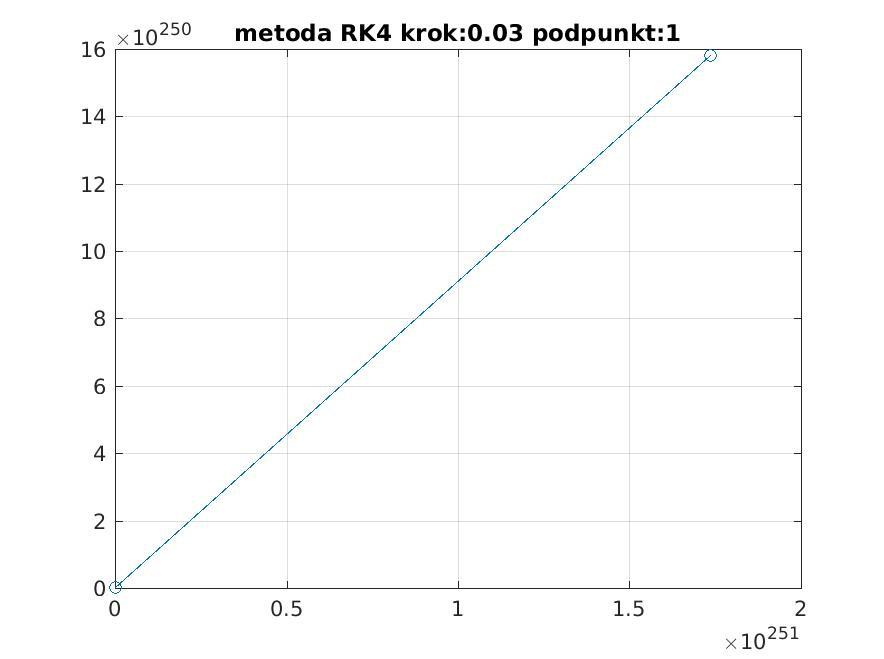
\includegraphics[width = 15cm]{2d/metoda RK4 krok:0,03 podpunkt:1.jpg}
\end{figure}

\begin{figure}[htp]
\centering
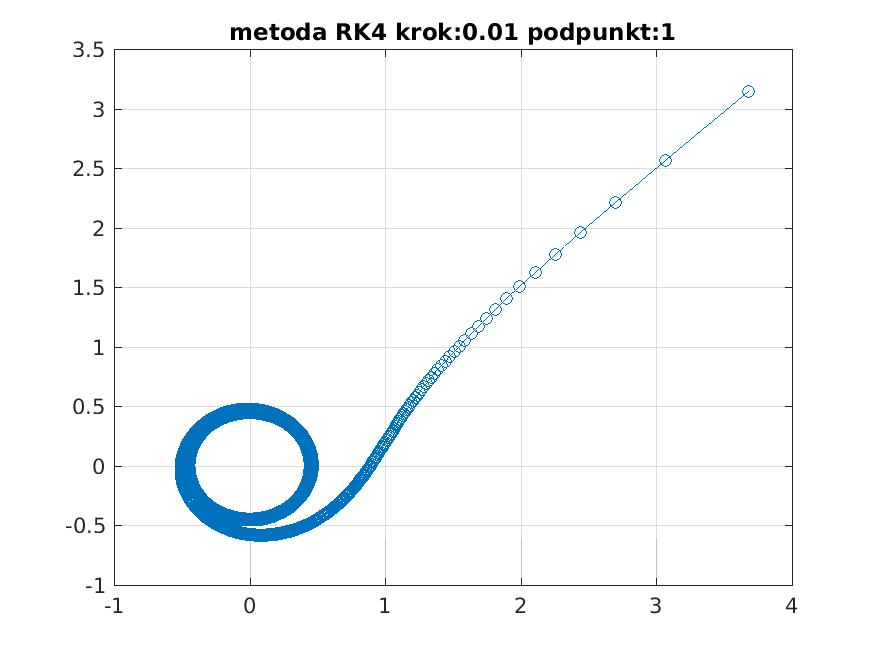
\includegraphics[width = 15cm]{2d/metoda RK4 krok:0,01 podpunkt:1.jpg}
\end{figure}

\begin{figure}[htp]
\centering
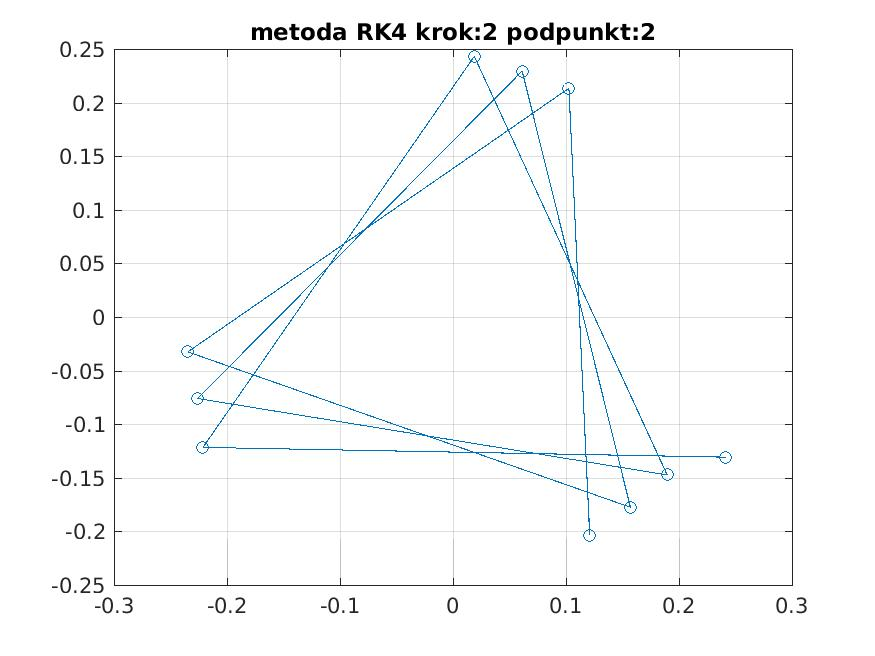
\includegraphics[width = 15cm]{2d/metoda RK4 krok:2 podpunkt:2.jpg}
\end{figure}

\begin{figure}[htp]
\centering
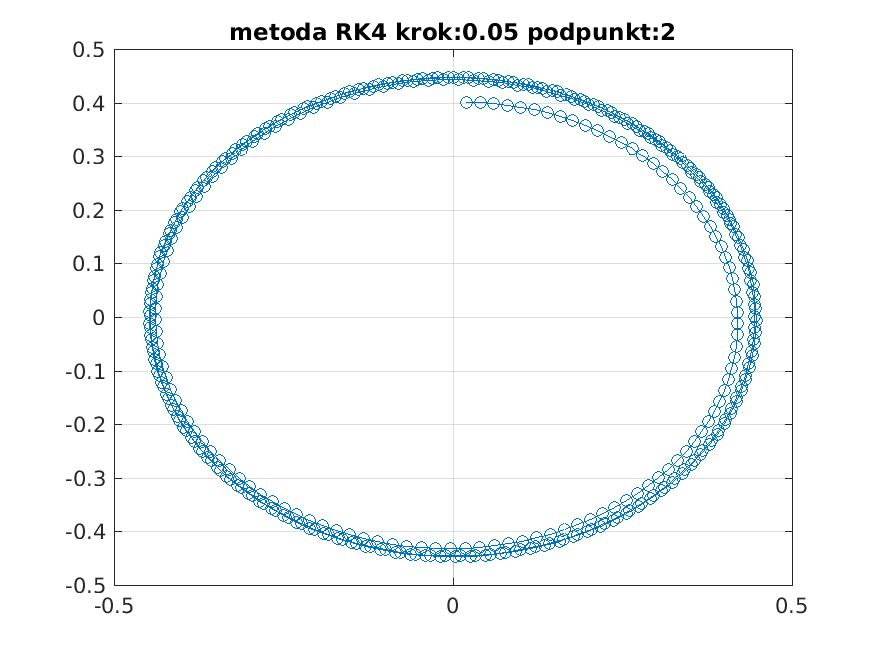
\includegraphics[width = 15cm]{2d/metoda RK4 krok:0,05 podpunkt:2.jpg}
\end{figure}

\begin{figure}[htp]
\centering
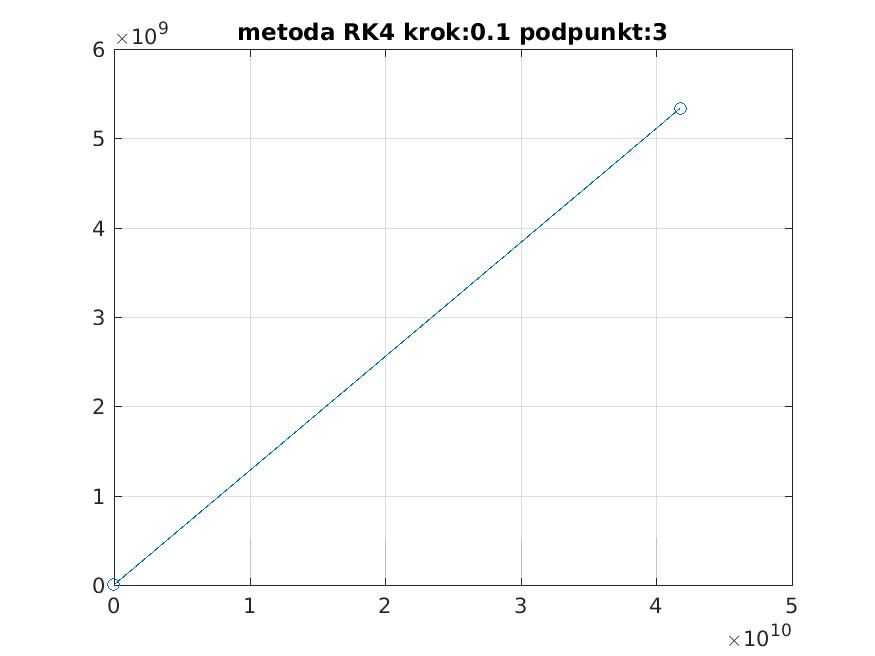
\includegraphics[width = 15cm]{2d/metoda RK4 krok:0,1 podpunkt:3.jpg}
\end{figure}

\begin{figure}[htp]
\centering
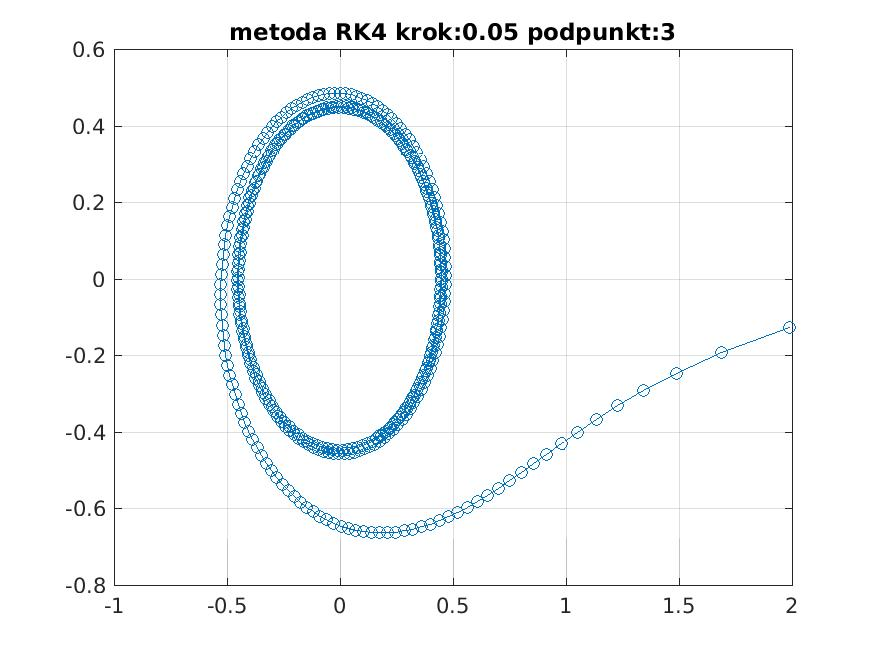
\includegraphics[width = 15cm]{2d/metoda RK4 krok:0,05 podpunkt:3.jpg}
\end{figure}

\begin{figure}[htp]
\centering
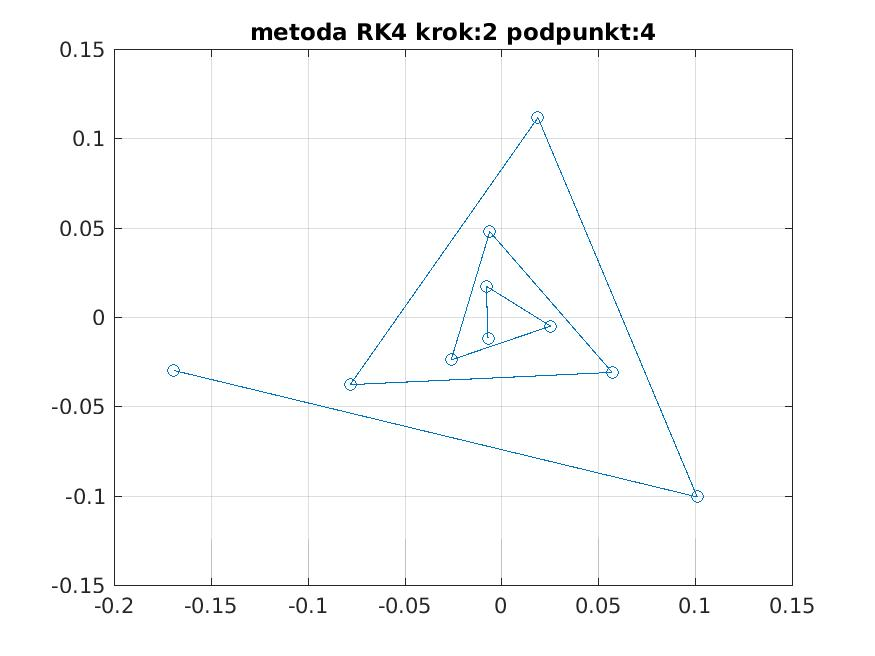
\includegraphics[width = 15cm]{2d/metoda RK4 krok:2 podpunkt:4.jpg}
\end{figure}

\begin{figure}[htp]
\centering
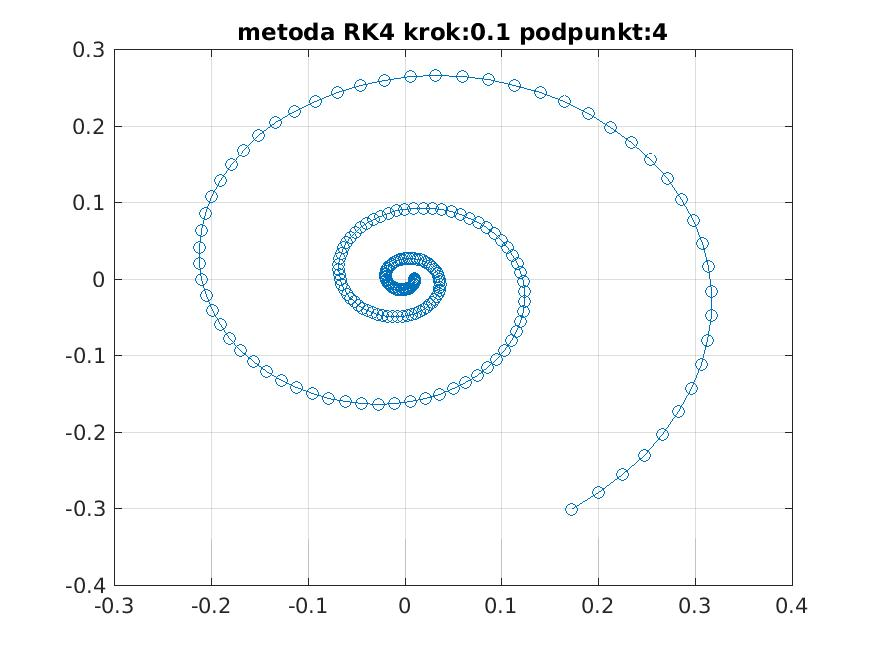
\includegraphics[width = 15cm]{2d/metoda RK4 krok:0,1 podpunkt:4.jpg}
\end{figure}

\subsection{Wnioski}
Metoda Rungego-Kutty dla podanych równań jest szybka i stabilna numeryczie przy odpowiednim kroku. Zmniejszając krok możaby coraz dokładniej wyznaczyć trajektorię. Dobór odpowiedniej długości kroku w sposób interaktywny jest problematyczny. Metoda róznież ma dość wysoki nakład obliczeniowy ponieważ jest on zależny tylko od przedziału i długości kroku, dlatego nie ma znaczenia czy równania są skomplikowane czy bardzo proste. 

\section{Metoda predyktor-korektor Adamsa ze stałym krokiem}
\subsection{Opis algorytmu}
Metoda predyktor-korektor Adamsa należy do grupy metod wielkorokowych..

\subsection{Realizacja funkcji RK4 w programie Matlab}
\begin{lstlisting}

\end{lstlisting}




\end{document}


